\documentclass{beamer}

% xcolor and define colors -------------------------
\usepackage{xcolor}

% https://www.viget.com/articles/color-contrast/
\definecolor{purple}{HTML}{5601A4}
\definecolor{navy}{HTML}{0D3D56}
\definecolor{ruby}{HTML}{9a2515}
\definecolor{alice}{HTML}{107895}
\definecolor{daisy}{HTML}{EBC944}
\definecolor{coral}{HTML}{F26D21}
\definecolor{kelly}{HTML}{829356}
\definecolor{cranberry}{HTML}{E64173}
\definecolor{jet}{HTML}{131516}
\definecolor{asher}{HTML}{555F61}
\definecolor{slate}{HTML}{314F4F}

% Mixtape Sessions
\definecolor{picton-blue}{HTML}{00b7ff}
\definecolor{violet-red}{HTML}{ff3881}
\definecolor{sun}{HTML}{ffaf18}
\definecolor{electric-violet}{HTML}{871EFF}

% Main theme colors
\definecolor{accent}{RGB}{17,59,99} 
\definecolor{accent2}{RGB}{245,159,24}
\definecolor{gray100}{HTML}{f3f4f6}
\definecolor{gray800}{HTML}{1F292D}

% UdeC Colors
\definecolor{UDECGold}{RGB}{245,159,24}
\definecolor{UDECBlue}{RGB}{17,59,99} 

% Beamer Options -------------------------------------

% Background
\setbeamercolor{background canvas}{bg = white}

% Change text margins
\setbeamersize{text margin left = 15pt, text margin right = 15pt} 

% \alert
\setbeamercolor{alerted text}{fg = UDECGold}

% Frame title
\setbeamercolor{frametitle}{bg = white, fg = jet}
\setbeamercolor{framesubtitle}{bg = white, fg = UDECBlue}
\setbeamerfont{framesubtitle}{size = \small, shape = \itshape}

% Block
\setbeamercolor{block title}{fg = white, bg = accent2}
\setbeamercolor{block body}{fg = gray800, bg = gray100}

% Title page
\setbeamercolor{title}{fg = gray800}
\setbeamercolor{subtitle}{fg = UDECBlue}

%% Custom \maketitle and \titlepage
\setbeamertemplate{title page}
{
    %\begin{centering}
        \vspace{20mm}
        {\Large \usebeamerfont{title}\usebeamercolor[fg]{title}\inserttitle}\\
        {\large \itshape \usebeamerfont{subtitle}\usebeamercolor[fg]{subtitle}\insertsubtitle}\\ \vspace{10mm}
        {\insertauthor}\\
        {\color{asher}\small{\insertdate}}\\
    %\end{centering}
}

% Table of Contents
\setbeamercolor{section in toc}{fg = UDECBlue!70!jet}
\setbeamercolor{subsection in toc}{fg = jet}

% Button 
\setbeamercolor{button}{bg = UDECBlue}

% Remove navigation symbols
\setbeamertemplate{navigation symbols}{}

% Table and Figure captions
\setbeamercolor{caption}{fg=jet!70!white}
\setbeamercolor{caption name}{fg=jet}
\setbeamerfont{caption name}{shape = \itshape}

% Bullet points

%% Fix left-margins
\settowidth{\leftmargini}{\usebeamertemplate{itemize item}}
\addtolength{\leftmargini}{\labelsep}

%% enumerate item color
\setbeamercolor{enumerate item}{fg = accent}
\setbeamerfont{enumerate item}{size = \small}
\setbeamertemplate{enumerate item}{\insertenumlabel.}

%% itemize
\setbeamercolor{itemize item}{fg = accent!70!white}
\setbeamerfont{itemize item}{size = \small}
\setbeamertemplate{itemize item}[circle]

%% right arrow for subitems
\setbeamercolor{itemize subitem}{fg = accent!60!white}
\setbeamerfont{itemize subitem}{size = \small}
\setbeamertemplate{itemize subitem}{$\rightarrow$}

\setbeamertemplate{itemize subsubitem}[square]
\setbeamercolor{itemize subsubitem}{fg = jet}
\setbeamerfont{itemize subsubitem}{size = \small}

% Special characters

\usepackage{collectbox}

\makeatletter
\newcommand{\mybox}{%
    \collectbox{%
        \setlength{\fboxsep}{1pt}%
        \fbox{\BOXCONTENT}%
    }%
}
\makeatother






% Links ----------------------------------------------

\usepackage{hyperref}
\hypersetup{
  colorlinks = true,
  linkcolor = accent2,
  filecolor = accent2,
  urlcolor = accent2,
  citecolor = accent2,
}


% Line spacing --------------------------------------
\usepackage{setspace}
\setstretch{1.2}


% \begin{columns} -----------------------------------
\usepackage{multicol}


% Fonts ---------------------------------------------
% Beamer Option to use custom fonts
\usefonttheme{professionalfonts}

% \usepackage[utopia, smallerops, varg]{newtxmath}
% \usepackage{utopia}
\usepackage[sfdefault,light]{roboto}

% Small adjustments to text kerning
\usepackage{microtype}



% Remove annoying over-full box warnings -----------
\vfuzz2pt 
\hfuzz2pt


% Table of Contents with Sections
\setbeamerfont{myTOC}{series=\bfseries, size=\Large}
\AtBeginSection[]{
        \frame{
            \frametitle{Roadmap}
            \tableofcontents[current]   
        }
    }


% Tables -------------------------------------------
% Tables too big
% \begin{adjustbox}{width = 1.2\textwidth, center}
\usepackage{adjustbox}
\usepackage{array}
\usepackage{threeparttable, booktabs, adjustbox}
    
% Fix \input with tables
% \input fails when \\ is at end of external .tex file
\makeatletter
\let\input\@@input
\makeatother

% Tables too narrow
% \begin{tabularx}{\linewidth}{cols}
% col-types: X - center, L - left, R -right
% Relative scale: >{\hsize=.8\hsize}X/L/R
\usepackage{tabularx}
\newcolumntype{L}{>{\raggedright\arraybackslash}X}
\newcolumntype{R}{>{\raggedleft\arraybackslash}X}
\newcolumntype{C}{>{\centering\arraybackslash}X}

% Figures

% \imageframe{img_name} -----------------------------
% from https://github.com/mattjetwell/cousteau
\newcommand{\imageframe}[1]{%
    \begin{frame}[plain]
        \begin{tikzpicture}[remember picture, overlay]
            \node[at = (current page.center), xshift = 0cm] (cover) {%
                \includegraphics[keepaspectratio, width=\paperwidth, height=\paperheight]{#1}
            };
        \end{tikzpicture}
    \end{frame}%
}

% subfigures
\usepackage{subfigure}


% Highlight slide -----------------------------------
% \begin{transitionframe} Text \end{transitionframe}
% from paulgp's beamer tips
\newenvironment{transitionframe}{
    \setbeamercolor{background canvas}{bg=accent!40!black}
    \begin{frame}\color{accent!10!white}\LARGE\centering
}{
    \end{frame}
}


% Table Highlighting --------------------------------
% Create top-left and bottom-right markets in tabular cells with a unique matching id and these commands will outline those cells
\usepackage[beamer,customcolors]{hf-tikz}
\usetikzlibrary{calc}
\usetikzlibrary{fit,shapes.misc}

% To set the hypothesis highlighting boxes red.
\newcommand\marktopleft[1]{%
    \tikz[overlay,remember picture] 
        \node (marker-#1-a) at (0,1.5ex) {};%
}
\newcommand\markbottomright[1]{%
    \tikz[overlay,remember picture] 
        \node (marker-#1-b) at (0,0) {};%
    \tikz[accent!80!jet, ultra thick, overlay, remember picture, inner sep=4pt]
        \node[draw, rectangle, fit=(marker-#1-a.center) (marker-#1-b.center)] {};%
}
\usepackage{breqn} % Breaks lines

\usepackage{amsmath}
\usepackage{mathtools}

\usepackage{pdfpages} % \includepdf

\usepackage{listings} % R code
\usepackage{verbatim} % verbatim

% Video stuff
\usepackage{media9}



% packages for bibs and cites
\usepackage{natbib}
\usepackage{har2nat}
\newcommand{\possessivecite}[1]{\citeauthor{#1}'s \citeyearpar{#1}}
\usepackage{breakcites}
\usepackage{alltt}

% tikz
\usepackage{tikz}
\usepackage{pgfplots}
\usetikzlibrary{calc, positioning, decorations.pathreplacing, arrows.meta, intersections}
\pgfdeclarelayer{bg}
\pgfdeclarelayer{back}
\pgfdeclarelayer{fg}
\pgfsetlayers{bg,main,fg,back}
\usetikzlibrary{shapes,arrows}

% Setup math operators
\DeclareMathOperator{\E}{E} \DeclareMathOperator{\tr}{tr} \DeclareMathOperator{\se}{se} \DeclareMathOperator{\I}{I} \DeclareMathOperator{\sign}{sign} \DeclareMathOperator{\supp}{supp} \DeclareMathOperator{\plim}{plim}
\DeclareMathOperator*{\dlim}{\mathnormal{d}\mkern2mu-lim}
\newcommand\independent{\protect\mathpalette{\protect\independenT}{\perp}}
   \def\independenT#1#2{\mathrel{\rlap{$#1#2$}\mkern2mu{#1#2}}}
\newcommand*\colvec[1]{\begin{pmatrix}#1\end{pmatrix}}

\newcommand{\myurlshort}[2]{\href{#1}{\textcolor{gray}{\textsf{#2}}}}


\title[Econometría II]{Econometría II}
\subtitle{Variables Instrumentales -- Causalidad}
\author[Felipe Quezada]{Felipe Quezada Escalona}
\date{(Slides de Scott Cunningham)}
%%%%%%%%%%%%%%%%%%%%%%%%%%%%%%%%%%%%%%%%%%%%%%
%%%%%%%%%%%%%%%%%%%%%%%%%%%%%%%%%%%%%%%%%%%%%%
\begin{document}
\begin{frame}[plain]
\begin{figure}
    \hspace{-8.75cm} \includegraphics[width=0.3\linewidth]{Images/depto_economía color.png}
    \textbf{}
\end{figure}
\vspace{-15pt}
\titlepage
\end{frame}


% ---- Content ----

\section{Estimadores}

\subsection{Efectos locales promedio del tratamiento}

\begin{frame}{Efectos del tratamiento constante vs heterogéneos}

\begin{itemize}
\item El IV se modeló utilizando resultados realizados, lo que dificultó la inferencia causal.
\item Pero también tendía a asumir efectos del tratamiento constantes.
\item Al introducir efectos del tratamiento heterogéneos, el IV se volvió más complejo.
\end{itemize}

\end{frame}

\begin{frame}{Algo de contexto}

\begin{itemize}
\item El Premio Nobel de Economía de octubre de 2021 fue para Card, Angrist e Imbens (los dos últimos por su trabajo de los años 90 sobre IV).
\item Angrist escribió una disertación utilizando instrumentos aleatorios (el draft de Vietnam), fue a Harvard, coincidió con Imbens durante un año, ambos fueron mentoreados por Gary Chamberlain, trabajaron con Don Rubin, y escribieron su famoso artículo sobre efecto promedio local del tratamiento (LATE).
\item Chamberlain recomendó modificar el marco de resultados potenciales de Rubin (en lugar de su modelado original de índice latente), lo que parece haber hecho el trabajo más atractivo de manera general (fuera de la economía).
\end{itemize}

\end{frame}

\begin{frame}{Concepto de tratamiento potencial}
	
El "estado de tratamiento potencial" ($D^j$) es como los resultados potenciales del experimento mental; no es el estado de tratamiento observado $D$ hasta que intercambiamos entre ellos con la asignación del instrumento.
\bigskip
		\begin{itemize}
		\item $D^1_{i} =$ el estado de tratamiento de $i$ cuando $Z_i=1$
		\item $D^0_{i} =$ el estado de tratamiento de $i$ cuando $Z_i=0$
		\end{itemize}
\bigskip
Representaremos los resultados como una función tanto del estado de tratamiento como del estado del instrumento. En otras palabras, $Y_i(D_i=0,Z_i=1)$ se representa como $Y_i(0,1)$.

\end{frame}

\begin{frame}{Identificación}
		
	\begin{enumerate}
	\item Suposición de Valor de Tratamiento Estable para las Unidades (SUTVA)
	\item Asignación aleatoria
	\item Restricción de exclusión
	\item Primera etapa distinta de cero
	\item Monotonía
	\end{enumerate}
\end{frame}


\begin{frame}{Efecto promedio local del tratamiento}

	Si se satisfacen todas las suposiciones del 1 al 5, entonces IV estima el \textbf{efecto promedio local del tratamiento (LATE)} de $D$ sobre $Y$: $$\delta_{IV,LATE} =\frac{\text{Efecto de Z sobre Y}}{\text{Efecto de Z sobre D}}$$

\end{frame}	



\begin{frame}{SUTVA en general}

  \begin{itemize}
    \item SUTVA significa ``supuesto de valor de tratamiento estable para las unidades''
          \begin{enumerate}
            \item \textbf{S}: \emph{\textbf{s}table} (estable)
            \item \textbf{U}: a través de todas las \emph{\textbf{u}nidades}, o la población
            \item \textbf{TV}: \emph{\textbf{t}reatment-value} (``efecto del tratamiento'', ``efecto causal'')
            \item \textbf{A}: \emph{\textbf{a}ssumption} (supuesto)
          \end{enumerate}
    \item Significa que un resultado potencial no tiene nada que ver con la asignación de tratamiento de otros: solo con la propia, y solo hoy.
  \end{itemize}
\end{frame}





\begin{frame}{SUTVA}

\begin{block}{SUTVA con respecto a IV}
En el contexto de IV, SUTVA significa que los \textbf{tratamientos potenciales} para cualquier unidad no (1) varían con los instrumentos asignados a otras unidades, y para cada unidad, (2) no hay diferentes formas o versiones de cada nivel del instrumento, que conduzcan a diferentes tratamientos potenciales.
\end{block}

\bigskip

Una vez que defines $D^1_i$, $D^0_i$ basado en un escalar, has invocado SUTVA, porque esto significa que tu resultado potencial no depende de la asignación de otros y que no hay variación oculta en el instrumento.

\bigskip

{\small\textbf{Ejemplo de violación a SUTVA:} El instrumento es un número de draft generado aleatoriamente. Cuando tu amigo, $i'$, es reclutado, tú, $i$, también eres reclutado, aunque no hayas sido asignado con tu número de draft.}
\end{frame}

\begin{frame}{Suposición de independencia}
	
	\begin{block}{Suposición de independencia}
	$\{Y_i(D^1_i,1),Y_i(D^0_i,0),D^1_{i},D^{0}_i\} \independent{Z}_i$
	\end{block}

\begin{itemize}	
\item Los instrumentos se asignan de manera independiente del estado de tratamiento potencial y de los resultados potenciales.
\item La independencia se asegura mediante la aleatorización física, pero quizás otras asignaciones también podrían hacerlo (por ejemplo, asignación alfabética).
\item Ejemplo: Números de draft aleatorios generados por un generador de números aleatorios.
\end{itemize}

\end{frame}

\begin{frame}{Independencia}

		 \textbf{Implicaciones de la independencia}: La primera etapa mide el efecto causal de $Z_i$ sobre $D_i$:
			\begin{eqnarray*}
			E[D_i|Z_i=1] - E[D_i|Z_i=0] &=& E[D^1_{i} | Z_i = 1] - E[D^0_{i}|Z_i = 0] \\
			&=& E[D^1_{i} - D^0_{i}]
			\end{eqnarray*}

\end{frame}

\begin{frame}{Independencia}

			 \textbf{Implicaciones de la independencia}: La forma reducida mide el efecto causal de $Z_i$ sobre $Y_i$:
			\begin{eqnarray*}
			E[Y_i | Z_i=1] - E[Y_i | Z_i=0] &=& E[Y_i(D^1_{i},1)|Z_i = 1] \\
			&& - E[Y_i(D^0_{i},0) | Z_i = 0] \\
			&=&E[Y_i(D^1_{i},1)] - E[Y_i(D^0_{i},0)]
			\end{eqnarray*}
			
			\bigskip
			
			Pero la independencia no es suficiente para que esto signifique que hemos identificado el efecto causal de $D$ sobre $Z$, ya que $Z$ podría estar operando directamente y no ``solo a través'' del tratamiento; para eso necesitamos la exclusión.
\end{frame}

\begin{frame}[plain]
\frametitle{Restricción de exclusión}

	\begin{block}{Restricción de exclusión}
	$\textbf{Y(D,Z)}=\textbf{Y(D,Z')}$ para todos $\textbf{Z}$, $\textbf{Z'}$, y para todos $\textbf{D}$
	\end{block}
	
\begin{itemize}
\item Observa cómo en la notación, $Z$ cambia a $Z'$, pero $D$ se mantiene fijo y, como resultado de mantenerse fijo, $Y$ no cambia.
\item Esa es la parte de ``solo a través de''. Cualquier efecto de $Z$ sobre $Y$ debe ser a través del efecto de $Z$ sobre $D$.
\item Recuerda el DAG y las \emph{flechas faltantes} de $Z$ a $\nu$ y de $Z$ a $Y$ directamente.
\item \textbf{Ejemplo de violación}: Tu número de draft te lleva a ir a la escuela de posgrado para evitar el reclutamiento, pero la escuela de posgrado cambia tus salarios; por lo tanto, la exclusión se viola incluso si el instrumento fue aleatorio.
\end{itemize}
	
\end{frame}

\begin{frame}[allowframebreaks]{Restricción de exclusión}
	
	\begin{itemize}
	\item Utiliza la restricción de exclusión para definir resultados potenciales indexados únicamente contra el estado de tratamiento (independientemente de la asignación del instrumento): 
		\begin{eqnarray*}
		 Y^1_{i} &=& Y_i(1,1) = Y_i(1,0) \\
		 Y^0_{i} &=& Y_i(0,1) = Y_i(0,0)
		\end{eqnarray*}
	\item Reescribe la ecuación de cambio:
		\begin{eqnarray*}
		Y_i &=& Y_i(0,Z_i) + [Y_i(1,Z_i) - Y_i(0,Z_i)]D_i \\
		Y_i &=& Y^0_{i} + [Y^1_{i} - Y^0_{i}]D_i \\
		Y_i &=& Y^0_i + \delta_iD_i
		\end{eqnarray*}
	\item Observa que aquí $D_i$ solo cambiará si la asignación del instrumento provoca que cambie, y así el efecto causal promedio capturado será solo para aquellos que responden a la asignación de su instrumento.
	\end{itemize}

\end{frame}


\begin{frame}[allowframebreaks]{Conoce tu mecanismo de asignación de tratamiento e instrumento}

Las personas tienden a apuntar a los argumentos de exclusión cuando los ven, porque, excepto en situaciones muy especiales como efectos de tratamiento homogéneos con sobreidentificación, se basan en suposiciones no verificables.

\bigskip

Angrist y Krueger (2001) señalan: ``En nuestra opinión, los buenos instrumentos a menudo provienen de un conocimiento detallado del mecanismo económico y de las instituciones que determinan el regressor de interés.''

\bigskip

Simplemente no puedes evitar la importancia de un profundo conocimiento del tratamiento y la asignación de instrumentos, ya que estos están literalmente en las suposiciones identificadoras (por ejemplo, independencia, exclusión).

\end{frame}


\begin{frame}[allowframebreaks]{Fuerte primera etapa}
	
	\begin{block}{Efecto causal promedio no nulo de $Z$ sobre $D$}
	$E[D^1_{i} - D^0_{i}]\neq{0}$
	\end{block}
				
\begin{itemize}
\item Recuerda la literatura sobre instrumentos débiles de antes (AR, $F$ muy grande).
\item $D^1$ significa que el instrumento está activado, y $D^0$ significa que está desactivado. Necesitamos que el tratamiento cambie cuando el instrumento cambia.
\item $Z$ tiene que tener algún efecto estadísticamente significativo sobre la probabilidad promedio de tratamiento.
\item Ejemplo: Verificar si un número de draft alto te hace más propenso a ser reclutado y viceversa.
\item Finalmente, una suposición verificable. Tenemos datos sobre $Z$ y $D$.
\end{itemize}

\end{frame}			


\begin{frame}{Monotonía}
	
	\begin{block}{Monotonía}
	O bien $\pi_{1i}\geq{0}$ para todos $i$, o $\pi_{1i}\leq{0}$ para todos $i=1, \dots, N$.
	\end{block}

\begin{itemize}

\item Recuerda que $\pi_{1i}$ es el efecto causal en forma reducida de la variable instrumental sobre el estado de tratamiento del individuo $i$.  
\item La monotonía requiere que la variable instrumental (débilmente) opere en la misma dirección sobre todas las unidades individuales.  
\item ``Cambiar el valor del instrumento no induce flujos bidireccionales dentro y fuera del tratamiento'' -- Michal Kolesar (2013).
\item Cualquiera afectado por el instrumento es afectado \emph{en la misma dirección} (es decir, positivamente o negativamente, pero no ambos).
\item \textbf{Ejemplo de una violación}: Las personas con un número de draft alto evitan el reclutamiento, pero se habrían ofrecido como voluntarios si hubieran obtenido un número bajo.

\end{itemize}

\end{frame}


\begin{frame}{Estimando}

	\vskip3pt plus.1fill
				
	Estimación de variables instrumentales (IV): 
	\begin{align*}
	\delta_{IV,LATE} & = \frac{E[Y_i(D^1_i, 1) - Y_i(D^0_i, 0)]}{E[D^1_i - D^0_i]}& \\
	& = E[(Y^1_i - Y^0_i) | D^1_i - D^0_i = 1]
	\end{align*}

\end{frame}		

\begin{frame}{Efecto Promedio Local del Tratamiento}
	
	\begin{itemize}
	\item El parámetro LATE es el efecto causal promedio de $D$ sobre $Y$ para aquellos cuyo estado de tratamiento fue cambiado por el instrumento, $Z$.
	\item Por ejemplo, IV estima el efecto promedio del servicio militar sobre los ingresos para la subpoblación que se enlistó en el servicio militar debido al reclutamiento, pero que no habría servido de otro modo. 
	\item LATE no nos dice cuál fue el efecto causal del servicio militar para los patriotas (voluntarios) o aquellos que fueron exentos del servicio militar por razones médicas. 
	\end{itemize}
	
\end{frame}


\begin{frame}{LATE y subpoblaciones}
	
IV estima el efecto promedio del tratamiento solo para una de estas subpoblaciones:
		\begin{enumerate}
		\item \underline{Siempre receptores}: Mi familia siempre ha servido, así que sirvo independientemente de si soy reclutado.
		\item \underline{Nunca receptores}: Soy objetor de conciencia, así que bajo ninguna circunstancia serviré, incluso si soy reclutado.
		\item \underline{Desafiadores}: Cuando fui reclutado, evadí. Pero si no me hubieran reclutado, habría servido. Soy un hombre de contradicciones.
		\item \textbf{Cumplidores}: Solo me inscribí en el ejército porque fui reclutado, de otro modo no habría servido.
		\end{enumerate}
\end{frame}


\begin{frame}[plain]
	\begin{columns}[t]
	\scriptsize
	\column{.4\textwidth}
	\begin{block}{Nunca Receptores}
		$D^1_i - D^0_i = 0$ \\
		$Y_i(0,1) - Y_i(0,0) = 0$ \\
		Por \textcolor{red}{Restricción de Exclusión}, el efecto causal de $Z$ sobre $Y$ es cero.
	\end{block}
	\begin{block}{Desafiador}
		$D^1_i - D^0_i = -1$ \\
		$Y_i(0,1) - Y_i(1,0) = Y_i(0) - Y_i(1)$ \\
		Por \textcolor{red}{Monotonía}, no hay nadie en este grupo.
	\end{block}
	\column{.4\textwidth}
	\begin{block}{Cumplidor}
		$D^1_i - D^0_i = 1$ \\
		$Y_i(1,1) - Y_i(0,0) = Y_i(1) - Y_i(0)$ \\
		Efecto Promedio del Tratamiento entre Cumplidores.
	\end{block}
	\begin{block}{Siempre Receptores}
		$D^1_i - D^0_i = 0$ \\
		$Y_i(1,1) - Y_i(1,0) = 0$ \\
		Por \textcolor{red}{Restricción de Exclusión}, el efecto causal de $Z$ sobre $Y$ es cero.
	\end{block}
	\end{columns}
\end{frame}


\begin{frame}{La Monotonía Asegura que no hay Desafiadores}
	
	\begin{itemize}
	\item ¿Por qué es importante no tener desafiadores?
		\begin{itemize}
		\item Si hubiera desafiadores, los efectos en los cumplidores podrían ser (en parte) cancelados por los efectos opuestos en los desafiadores.
		\item Se podría entonces observar una forma reducida cercana a cero, aunque los efectos del tratamiento sean positivos para todos (pero los cumplidores son impulsados en una dirección por el instrumento y los desafiadores en la dirección opuesta).
		\end{itemize}
	\item La monotonía asume que no hay desafiadores (hay versiones débiles y fuertes de esta suposición).
	\end{itemize}

\end{frame}

\begin{frame}{LATE no es el ATE}
	
	\begin{itemize}
	\item IV estima el efecto causal promedio para aquellas unidades afectadas por el instrumento (es decir, los efectos causales en los cumplidores).
	\item Trabajos a mediados de los años 2000 encontraron que con instrumentos continuos, podría ser posible extrapolar del LATE al parámetro agregado (literatura del efecto del tratamiento marginal).
	\item No se estudia acá, es importante aprenderla si quieren dedicarse a causalidad con IV.
	\end{itemize}

\end{frame}

		
\begin{frame}{Sensibilidad a las suposiciones: restricción de exclusión}
	
\begin{itemize}
	
\item Alguien en riesgo de ser reclutado (número bajo en la lotería) cambia sus planes de educación para mantener los aplazamientos del servicio militar y evitar el reclutamiento.

\item Aumento del sesgo en el estimador IV a través de dos canales:
		\begin{itemize}
		\item Efecto directo promedio de $Z$ sobre $Y$ para los cumplidores.
		\item Efecto directo promedio de $Z$ sobre $Y$ para los no cumplidores multiplicado por la probabilidad de ser un no cumplidor.
		\end{itemize}

\item La severidad depende de: 
		\begin{itemize}
		\item Probabilidad de no cumplimiento (menor $\rightarrow$ menos sesgo).
		\item "Fuerza" del instrumento (más fuerte $\rightarrow$ menos sesgo).
		\item Efecto del canal alternativo en $Y$.
		\end{itemize}
\end{itemize}

\end{frame}


\begin{frame}{Sensibilidad a las suposiciones: violaciones de monotonía}

\begin{itemize}

\item Alguien que se hubiera ofrecido como voluntario para el ejército cuando no estaba en riesgo de ser reclutado (número alto en la lotería) elige evitar el servicio militar cuando está en riesgo de ser reclutado (número bajo en la lotería).
	
\item Sesgo en el estimador IV (multiplicación de 2 términos):
		\begin{itemize}
		\item Proporción de desafiadores en relación con los cumplidores.
		\item Diferencia en los efectos causales promedio de $D$ sobre $Y$ para los cumplidores y desafiadores.
		\end{itemize}
\item La severidad depende de:
		\begin{itemize}
		\item Proporción de desafiadores (pequeña $\rightarrow$ menos sesgo).
		\item "Fuerza" del instrumento (más fuerte $\rightarrow$ menos sesgo).
		\item Variación en el efecto de $D$ sobre $Y$ (menor $\rightarrow$ menos sesgo).
		\end{itemize}
\end{itemize}
		
\end{frame}


	
		\section{Aplicación}

\subsection{Visualización de datos y evidencia necesaria}

\begin{frame}{Consejos prácticos}

\begin{itemize}
\item Antes de que pasemos a las aplicaciones, hablemos sobre imágenes
\item Es muy fácil que la inferencia causal se convierta en una caja negra, pero cuanto más lo sea, menos personas creerán en tu análisis
\item También hay evidencia reciente de que los trabajos de IV muestran signos de sesgo de publicación con un gran aumento en los valores $p$ alrededor de 0.05 (a diferencia de RCT y RDD)
\item Las imágenes son cruciales, pero son tipos particulares de imágenes las que necesitas mostrar para IV, en lo que quiero hacer hincapié (no cualquier visualización de datos)
\end{itemize}

\end{frame}

\begin{frame}{Mostrar Cantidades de Wald}

Presenta tus principales resultados como cantidades de Wald en hermosas imágenes de correlaciones simples, incluso si estás estimando con 2SLS
	\begin{itemize}
	\item Muestra imágenes de la \textcolor{blue}{primera etapa}. Si no puedes ver la correlación en la primera etapa, tienes un problema de instrumento débil
	\item Muestra en su lugar imágenes de la \textcolor{blue}{forma reducida}. Si no puedes ver la correlación en la forma reducida, es probable que no esté allí.
	\end{itemize}
	
	\bigskip
	
Esto puede ser un desafío ya que no todos los diseños de IV se prestan fácilmente a imágenes, por lo que ayuda familiarizarte con una gama de imágenes para obtener inspiración

\end{frame}

\begin{frame}{Consejos IV: Visualizando mi instrumento}
	
	\begin{figure}
	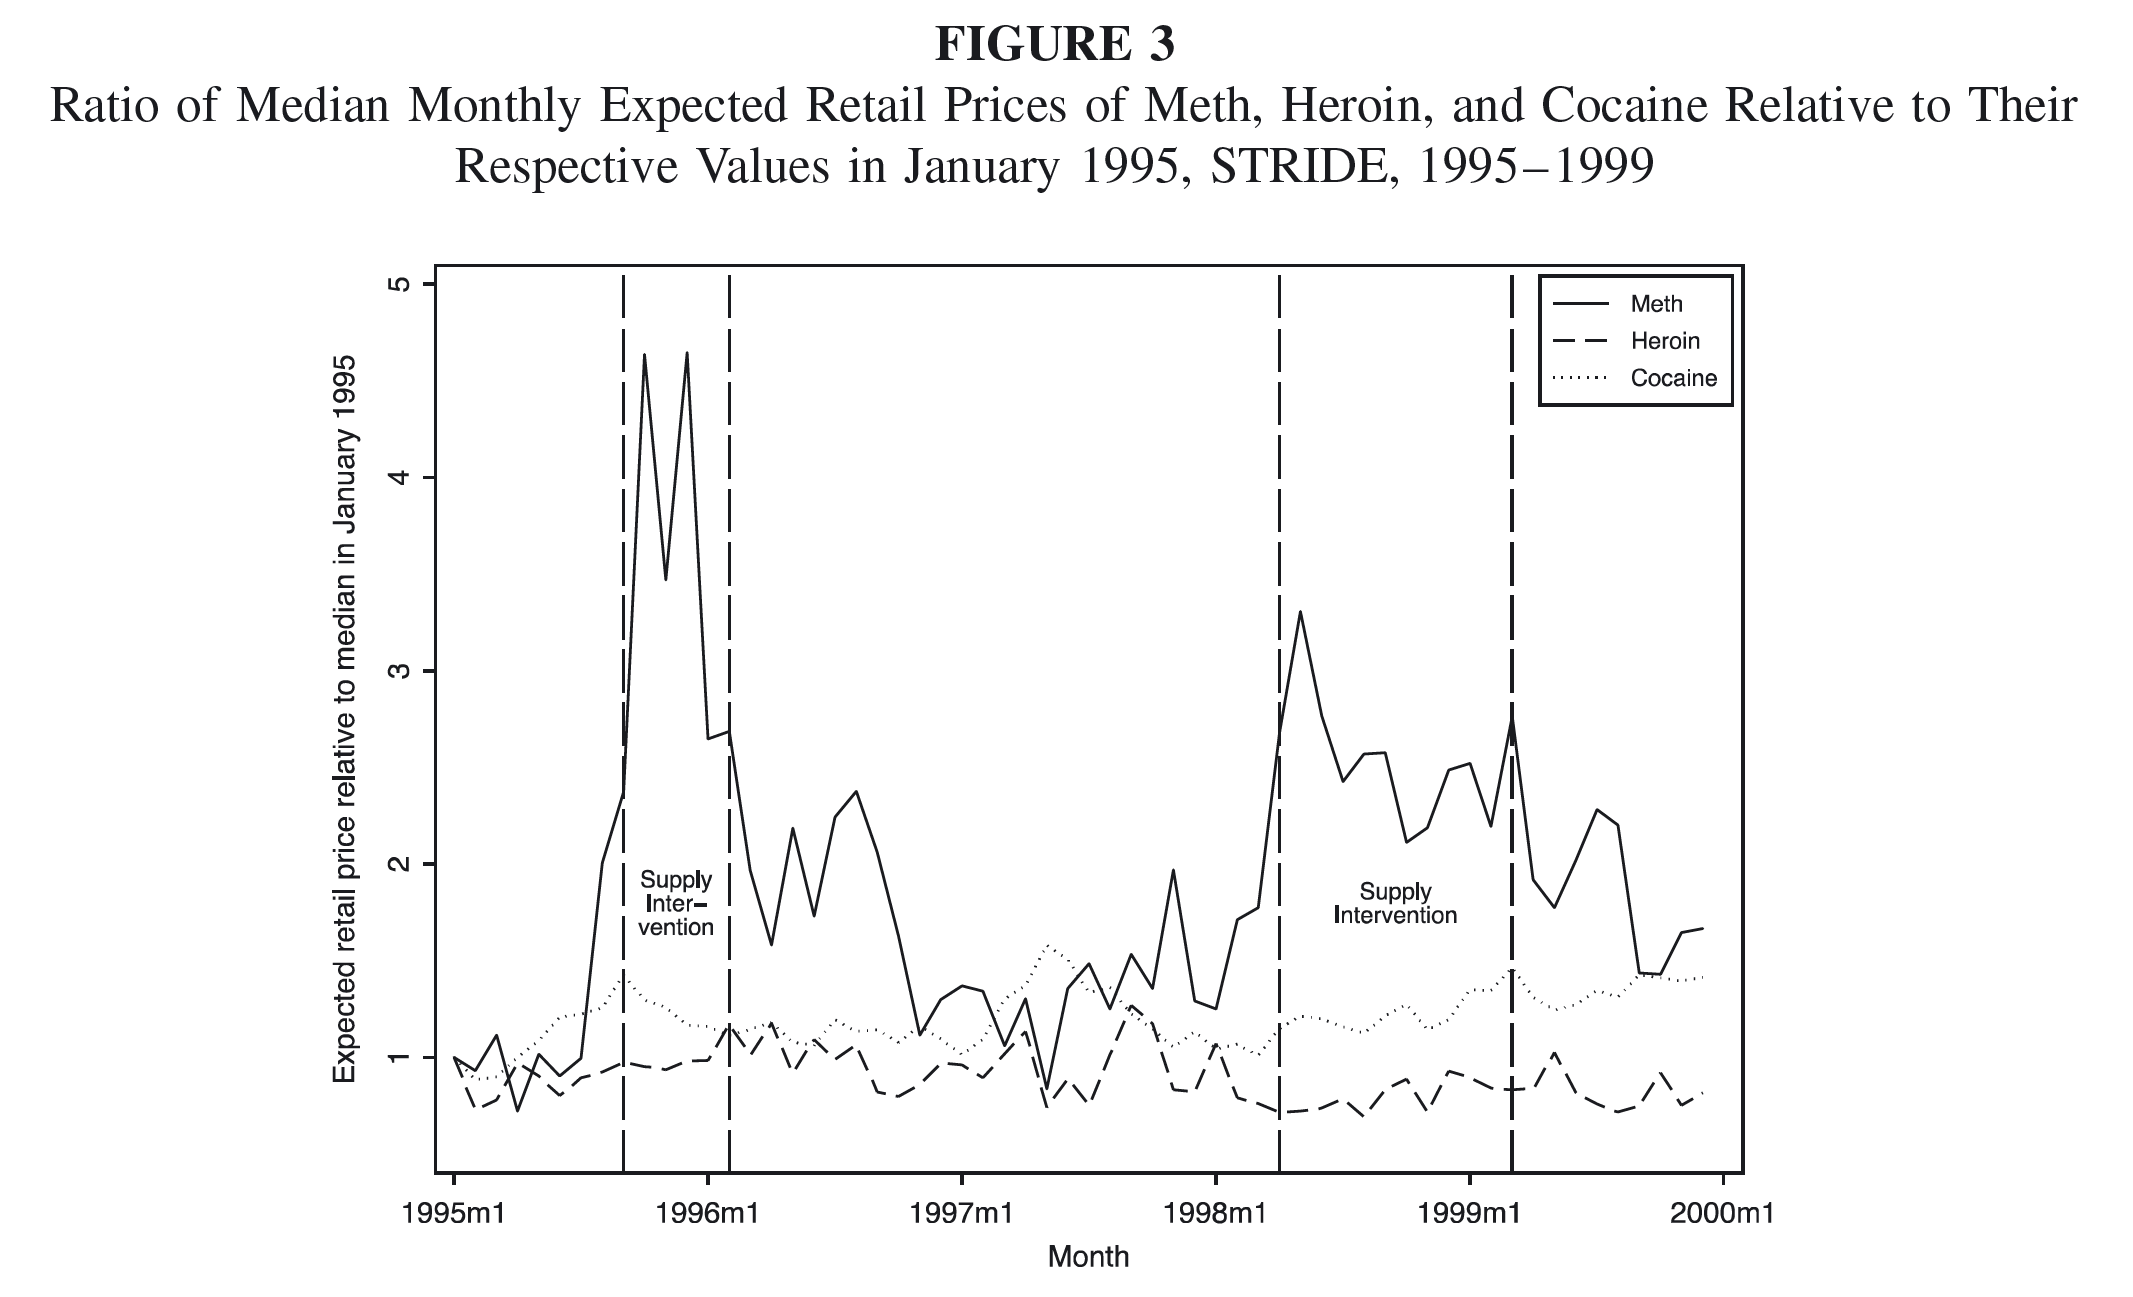
\includegraphics[scale=0.15]{./lecture_includes/keith_1.png}
	\end{figure}
	
\end{frame}

\begin{frame}{Consejos IV: Visualizando la primera etapa}
	
	\begin{figure}
	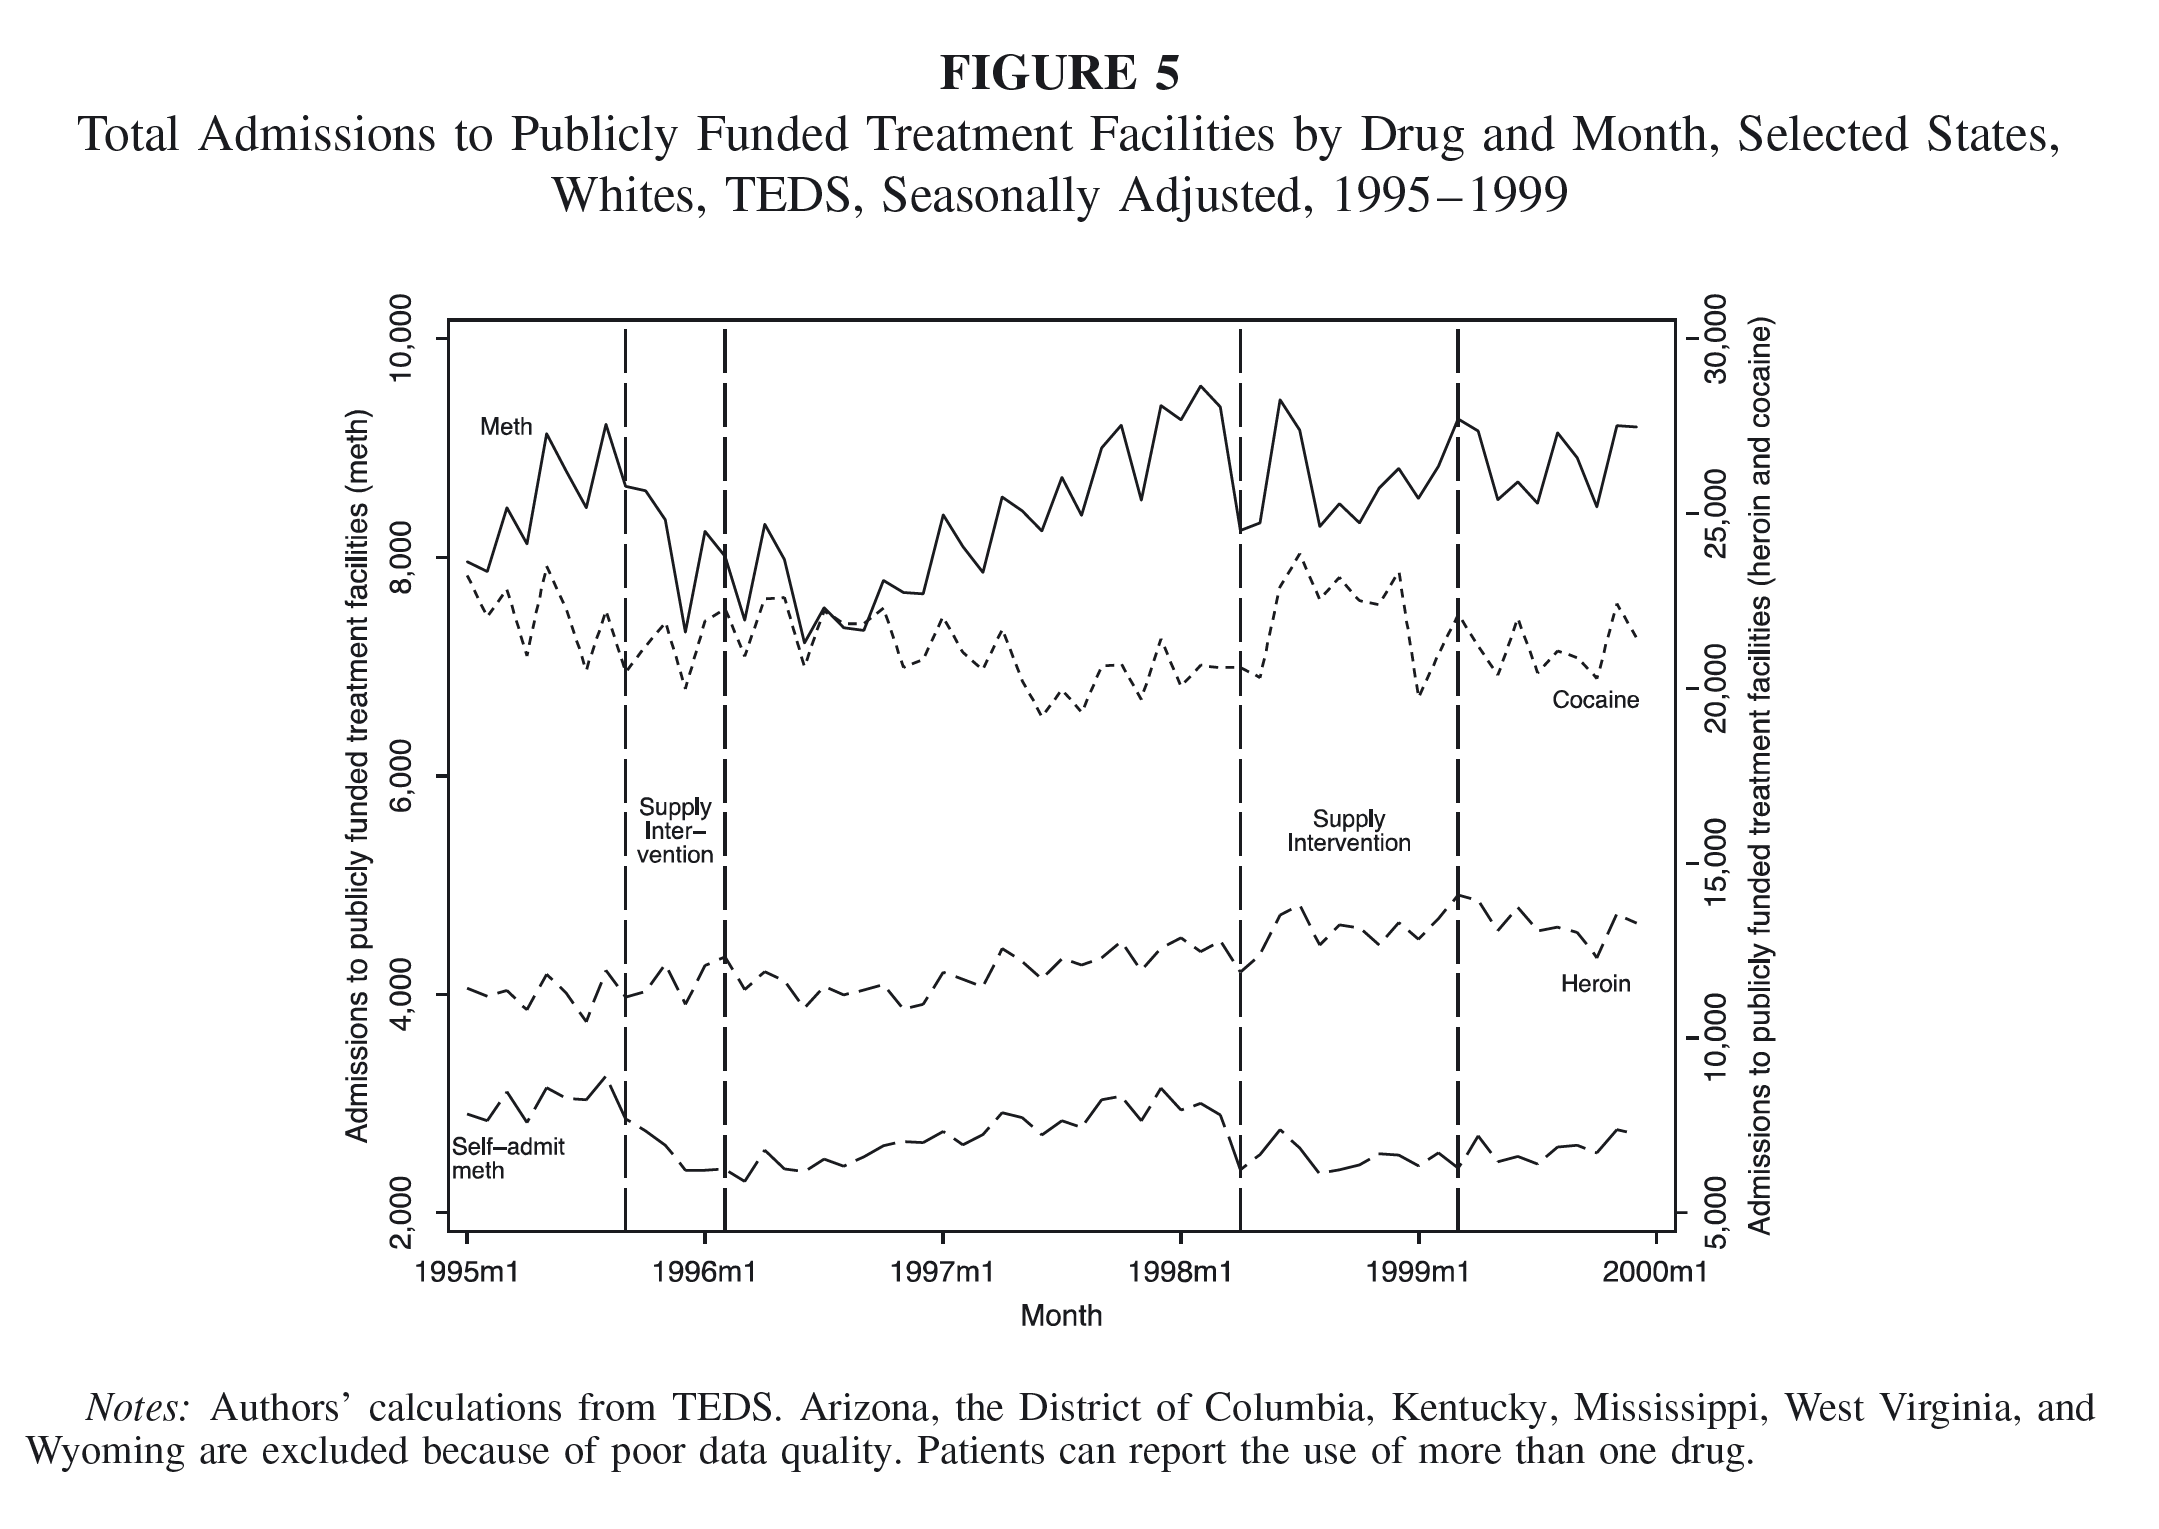
\includegraphics[scale=0.15]{./lecture_includes/keith_3.png}
	\end{figure}
	
\end{frame}

\begin{frame}{Consejos IV: Visualizando la forma reducida}
	
	\begin{figure}
	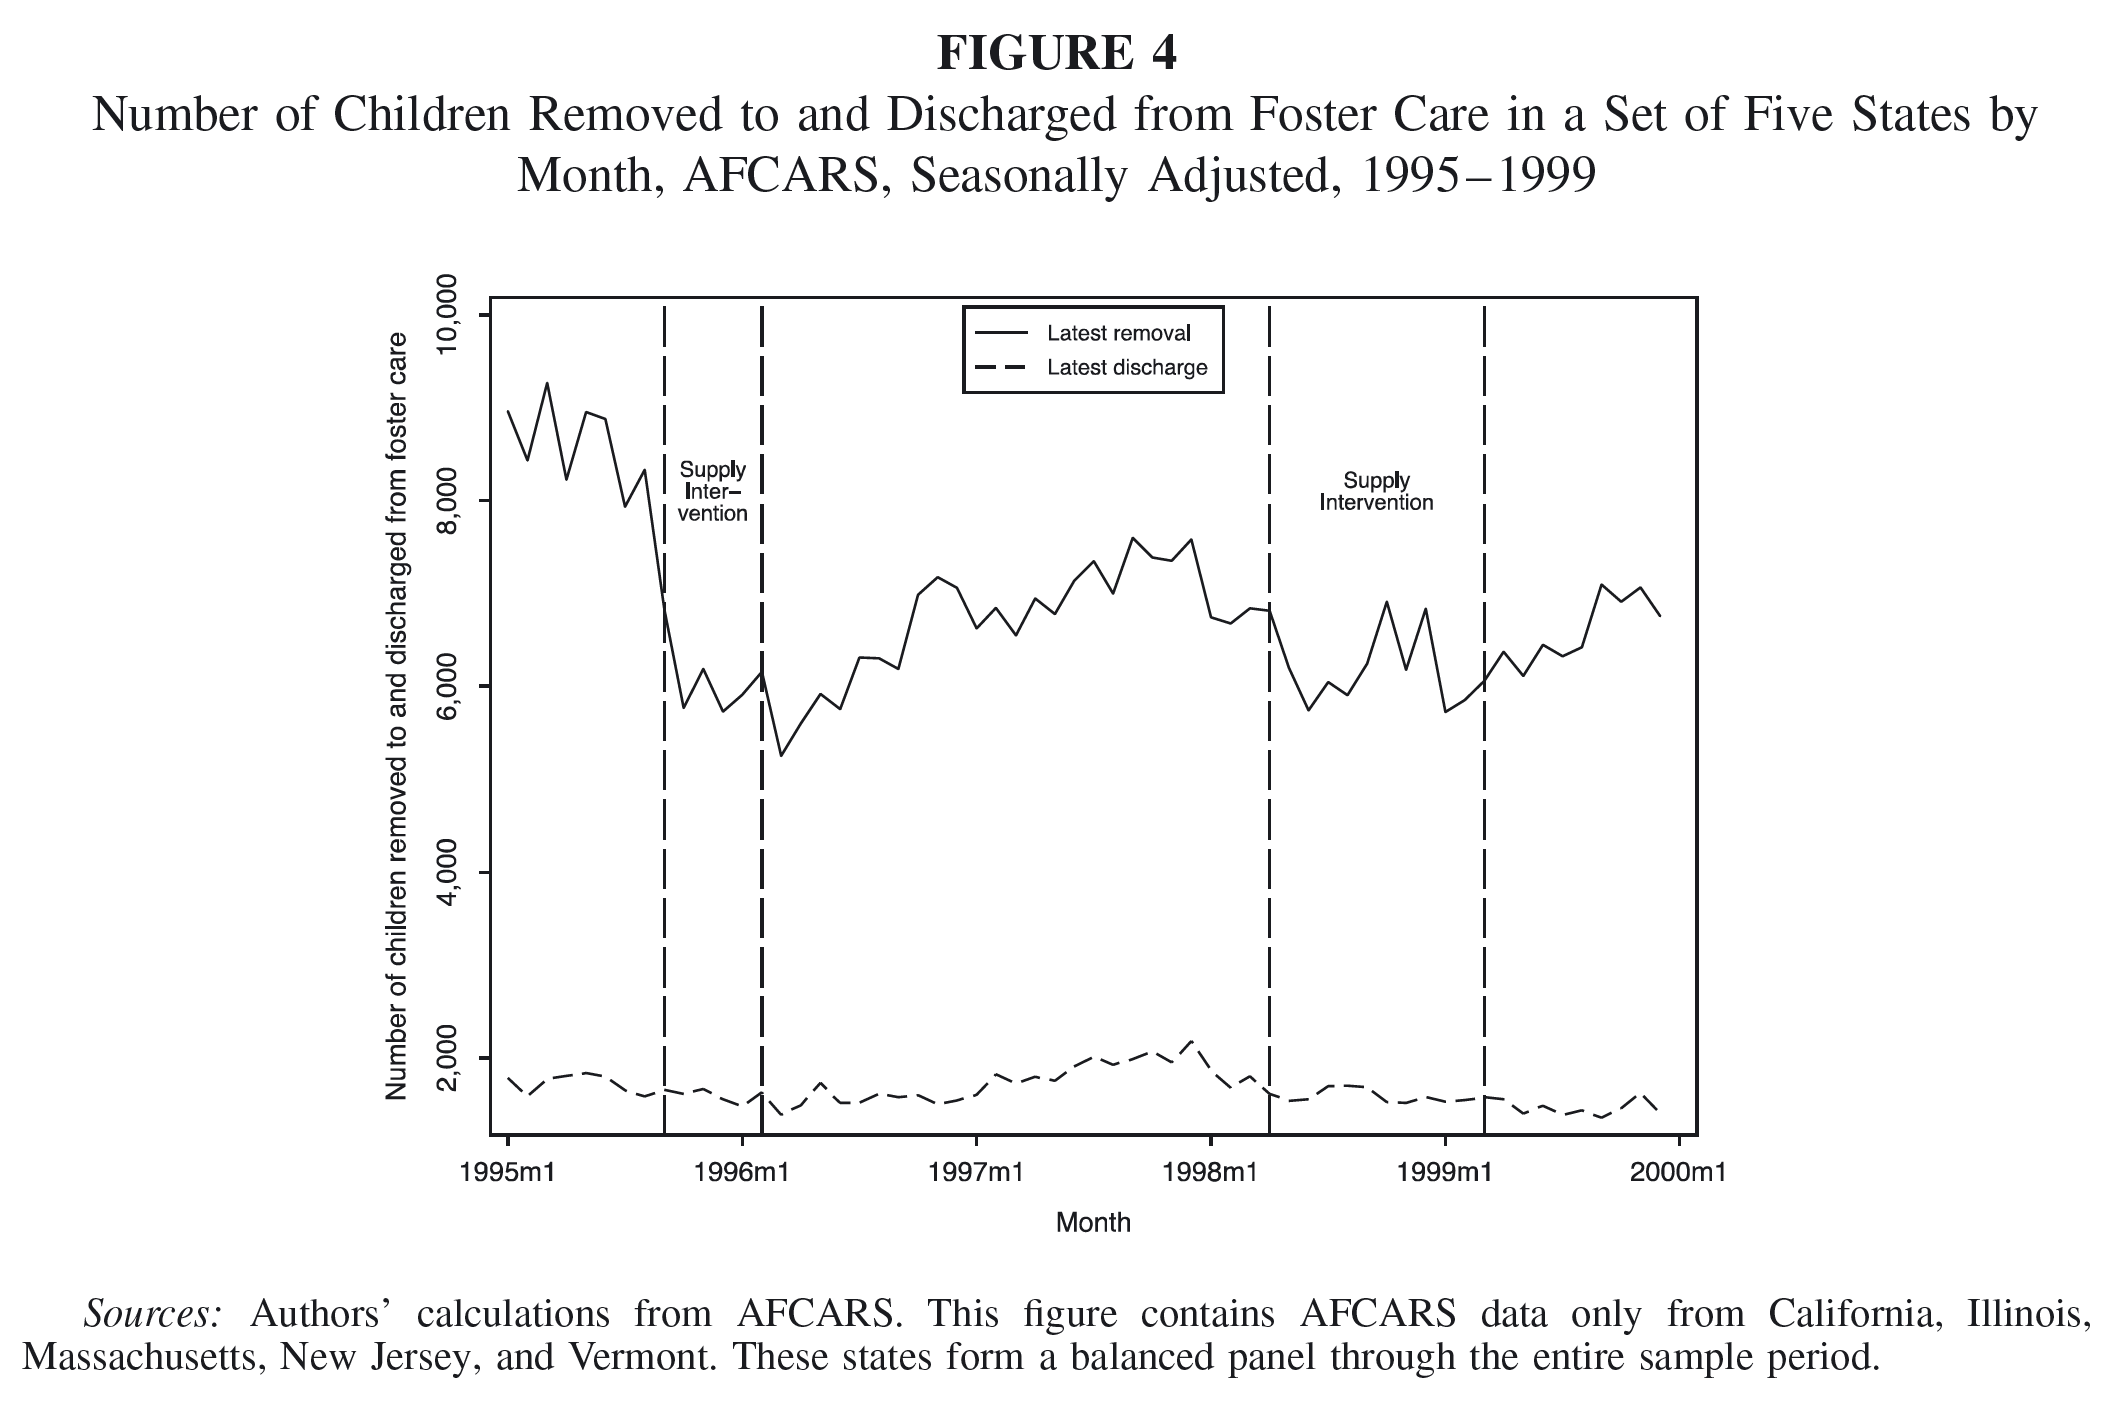
\includegraphics[scale=0.15]{./lecture_includes/keith_2.png}
	\end{figure}
	
\end{frame}

\begin{frame}{Tablas}

\begin{enumerate}
\item Modelo OLS ingenuo (aunque con heterogeneidad esto puede no ser informativo del mismo parámetro con IV)
\item Forma reducida
\item Primera etapa
\item Pruebas de instrumento débil
\item Modelo IV
\end{enumerate}

\end{frame}








\subsection{Elasticidad precio de la demanda}

\begin{frame}{Oferta y demanda}

\begin{itemize}
\item Las variables instrumentales se desarrollaron en los años 1920, en gran medida para abordar los problemas creados por la oferta y la demanda.
\item Las curvas de demanda son funciones causales, pero las curvas de oferta también lo son.
\item No observamos todos los precios y cantidades para poder calcular la pendiente o la forma de la curva de demanda porque solo observamos los "precios y cantidades realizados" en equilibrio.
\item Pero si supiéramos la elasticidad precio de la demanda, podríamos establecer políticas más óptimas como la política fiscal o la maximización de beneficios.
\end{itemize}

\end{frame}

\begin{frame}{Oferta y demanda}
	
	\begin{figure}
	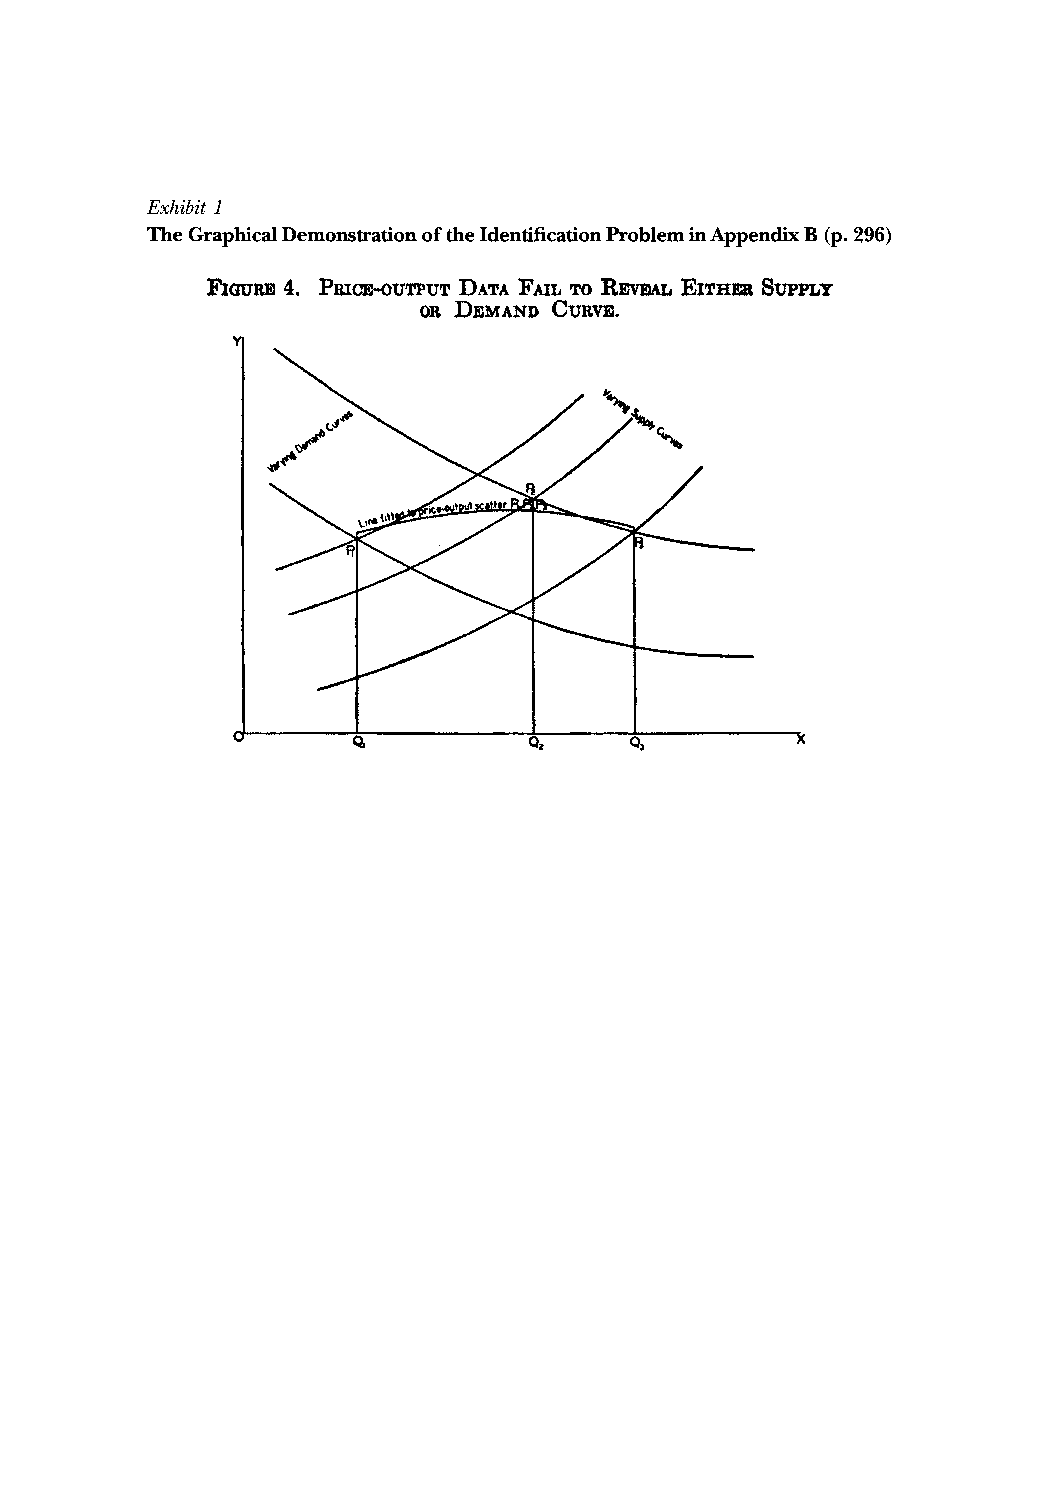
\includegraphics[scale=0.72]{./lecture_includes/supply_demand.pdf}
	\end{figure}
\end{frame}


\begin{frame}{Precio y cantidad iniciales}

	\begin{figure}
	\includegraphics[scale=0.15]{./lecture_includes/elasticity_1.jpg}
	\end{figure}
\end{frame}

\begin{frame}{Desplazamiento de la oferta}

	\begin{figure}
	\includegraphics[scale=0.15]{./lecture_includes/elasticity_2.jpg}
	\end{figure}
\end{frame}


\begin{frame}{Elasticidad precio de la demanda}

\begin{eqnarray*}
\delta = \frac{Q_2 - Q_1}{P_2 - P_1}
\end{eqnarray*}

\bigskip

Puede estimarse con regresiones log-log:

\bigskip

\begin{eqnarray*}
Ln Q_{it} = \alpha + \delta Ln P_{it} + \psi_{it}
\end{eqnarray*}

\bigskip

Pero necesitas un instrumento para el precio, y debe ser un desplazador de la oferta únicamente.

\end{frame}

\begin{frame}{Desplazamiento de la oferta}

\begin{itemize}
\item \textbf{Desplazadores de la oferta}: Los costos de insumos de la empresa y la tecnología son candidatos típicos.
\item \textcolor{red}{Desplazadores de la demanda}: Otros precios de bienes de consumo, ingreso del consumidor, disponibilidad de sustitutos, expectativas sobre el futuro.
\item Los buenos instrumentos deben desplazar \textbf{solo} la oferta -- \textcolor{red}{no la demanda}.
\end{itemize}

\end{frame}

\section{Conclusión}

\begin{frame}{Conclusión}

\begin{itemize}
\item ``Con una palanca lo suficientemente larga, puedo mover el mundo'' -- Arquímedes
\item Con un instrumento lo suficientemente fuerte y extraño, puedes identificar el LATE incluso fuera del laboratorio.
\item Necesitas saber qué buscar, así que ten en mente ese DAG todo el tiempo -- escríbelo en la pared.
\item Pero al igual que con la selección en observables, necesitamos supuestos plausibles, datos correctamente medidos y estimadores apropiados.
\end{itemize}

\end{frame}


\end{document}